\documentclass[aspectratio=169]{beamer}

\usepackage{caption}
\usepackage[utf8x]{inputenc}
\usepackage{graphicx}
\usepackage{textcomp}
\usepackage{tikz}
\usepackage{xcolor}
\usepackage{xmpmulti}

\graphicspath{{./images/}}
\makeatletter
\def\input@path{{./}{./images}}
\makeatother

\newcommand\imageright[1]{ %
    \caption*{\scalebox{.5}{\textcolor{lightgray}{\textcopyright~#1}}} %
}

\usetheme{HGF}

\title{Machine Learning with Neural Networks}
\subtitle{GridKa School 2018}
\author{Markus Götz}
\date{2018-08-29}
\institute{KIT}

\begin{document}
    
\section{Introduction}
\label{sec:introduction}

\maketitle

%%%%%%%%%%%%%%%%%%%%%%%%%%%%%%%%%%%%%%%%%%%%%%%%%%%%%%%%%%%%%%%%%%%%%%%%%%%
\begin{frame}
\frametitle{Outline}
    \tableofcontents[hideallsubsections]
\end{frame}

\section{Machine Learning Fundamentals}
\label{sec:machine-learning}

\subsection{Terminology}
\label{subsec:terminology}

\begin{frame}
    \frametitle{Terminology}
    \begin{figure}
        \centering
        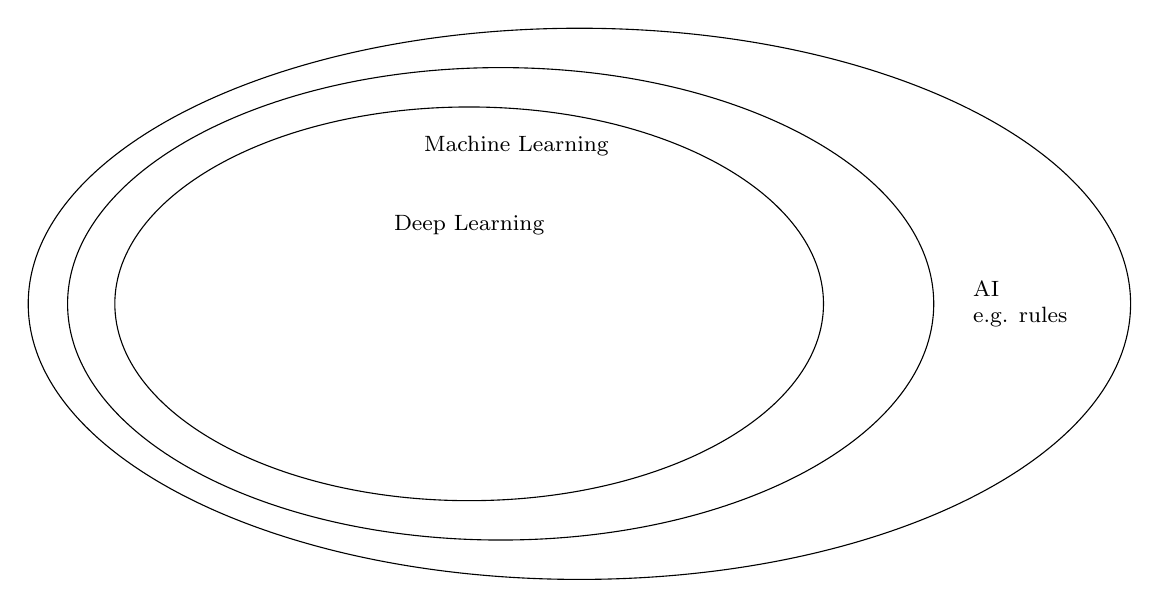
\begin{tikzpicture}[fill=white, font=\footnotesize]
            \draw (0, 0) ellipse (7.0 and 3.5);
            \node[align=left] at (5.6, 0.0) {AI\\e.g. rules};
            
            \draw (-1.0, 0) ellipse (5.5 and 3.0) (-0.8, 2.0) node {Machine Learning};
            
            \draw (-1.4, 0) ellipse (4.5 and 2.5) (-1.4, 1.0) node {Deep Learning};
        \end{tikzpicture}
    \end{figure}
\end{frame}

\begin{frame}
    \frametitle{Terminology}
    \begin{columns}
        \begin{column}{0.48\textwidth}
            \begin{itemize}
                \item \textbf{Samples}
                \item \textbf{Attributes}
                \item \textbf{Channels}
            \end{itemize}
        \end{column}
        \begin{column}{0.48\textwidth}
            \begin{figure}
                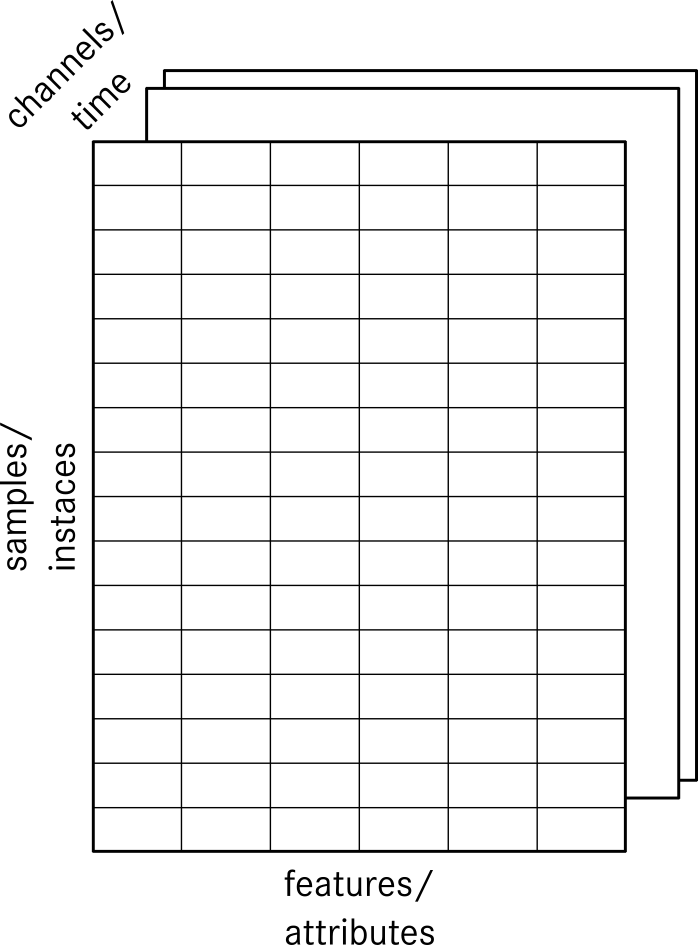
\includegraphics{terminology.png}
            \end{figure}
        \end{column}
    \end{columns}
\end{frame}


\begin{frame}
\frametitle{Terminology}
    \begin{itemize}
        \item \textbf{Supervised learning:} Learn by ``mimicking supervisor'', i.e. pattern annotations\\ 
        examples: image classification, stock forecasting
        \item \textbf{Unsupervised learning:} Determine patterns purely based on data\\ examples: customer cluster analysis, distribution estimation
        \item \textbf{Reinforcement learning:} Pavlov-style learning with punishment and reward in dynamic environments\\
        examples: game AIs, e.g. AlphaGo or Dota OpenAI
    \end{itemize}

    \medskip
\end{frame}


\subsection{Frameworks}

\subsection{Exercise: MNIST Dataset}

\begin{frame}
    \frametitle{Exercise 1: Warm-up}
    \begin{figure}
        \centering
        \begin{tikzpicture}[]
            \node [inner sep=0pt,above right] { %
                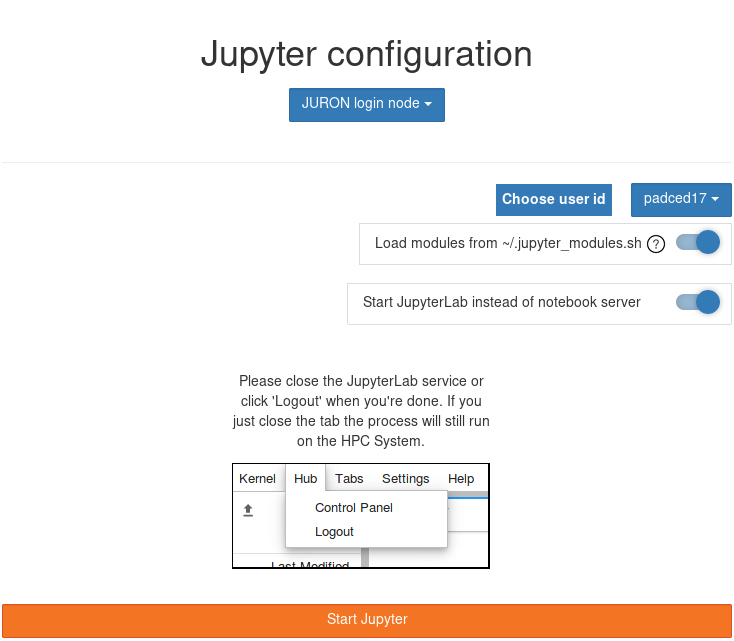
\includegraphics[width=0.5\linewidth]{jupyter.png} %
            };
            % show origin
            \draw [line width=0.6mm, red] (7.05, 4.05) ellipse (0.5 and 0.25);
        \end{tikzpicture}
    \end{figure}
\end{frame}

\subsection{Classification}
\subsection{Logistic Regression}

\subsection{Exercise: Logistic Regression}
\label{subsec:exercise-logistic-regression}

\begin{frame}
    \frametitle{Exercise: Logistic Regression}
    \begin{figure}
        \centering
    \end{figure}
\end{frame}

\section{Neural Networks}
\label{sec:neural-networks}

\subsection{Optimization}
\subsection{Generalization}

\subsection{Exercise: MNIST FNN}
\label{subsec:exercise-fnn}

\begin{frame}
    \frametitle{Exercise: MNIST Image Classification}
    
    \begin{figure}
        \centering
        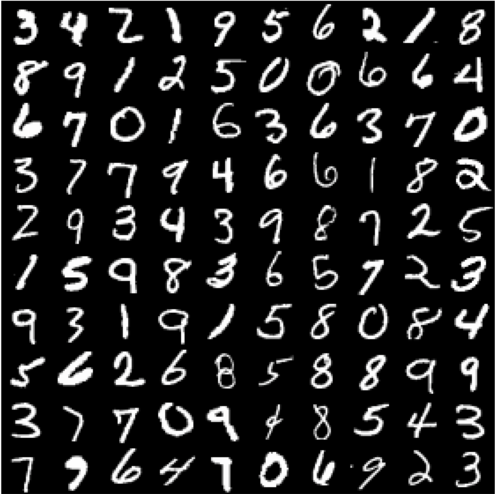
\includegraphics[width=0.4\linewidth]{mnist.png}
    \end{figure}
\end{frame}

\section{Convolutional Neural Networks}
\label{sec:convolutional-neural-networks}

\subsection{Discrete Convolution}
\label{subsec:discrete-convolution}

\begin{frame}
    \frametitle{Discrete Convolution}
    \begin{figure}
        \centering
        \multiinclude[<+->][format=png, graphics={width=0.8\linewidth}]{convolution}
        \imageright{Machine Learning Guru}
    \end{figure}
\end{frame}

\subsection{Network Architecture}
\subsection{Exercise: MNIST CNN}

\section{Regression}

\subsection{Discrete Convolutions}
\subsection{Network Architecture}
\subsection{Exercise: Abalone}

\begin{frame}
    \frametitle{Exercise: Abalone Age Regression Analysis}
    \begin{figure}
        \centering
        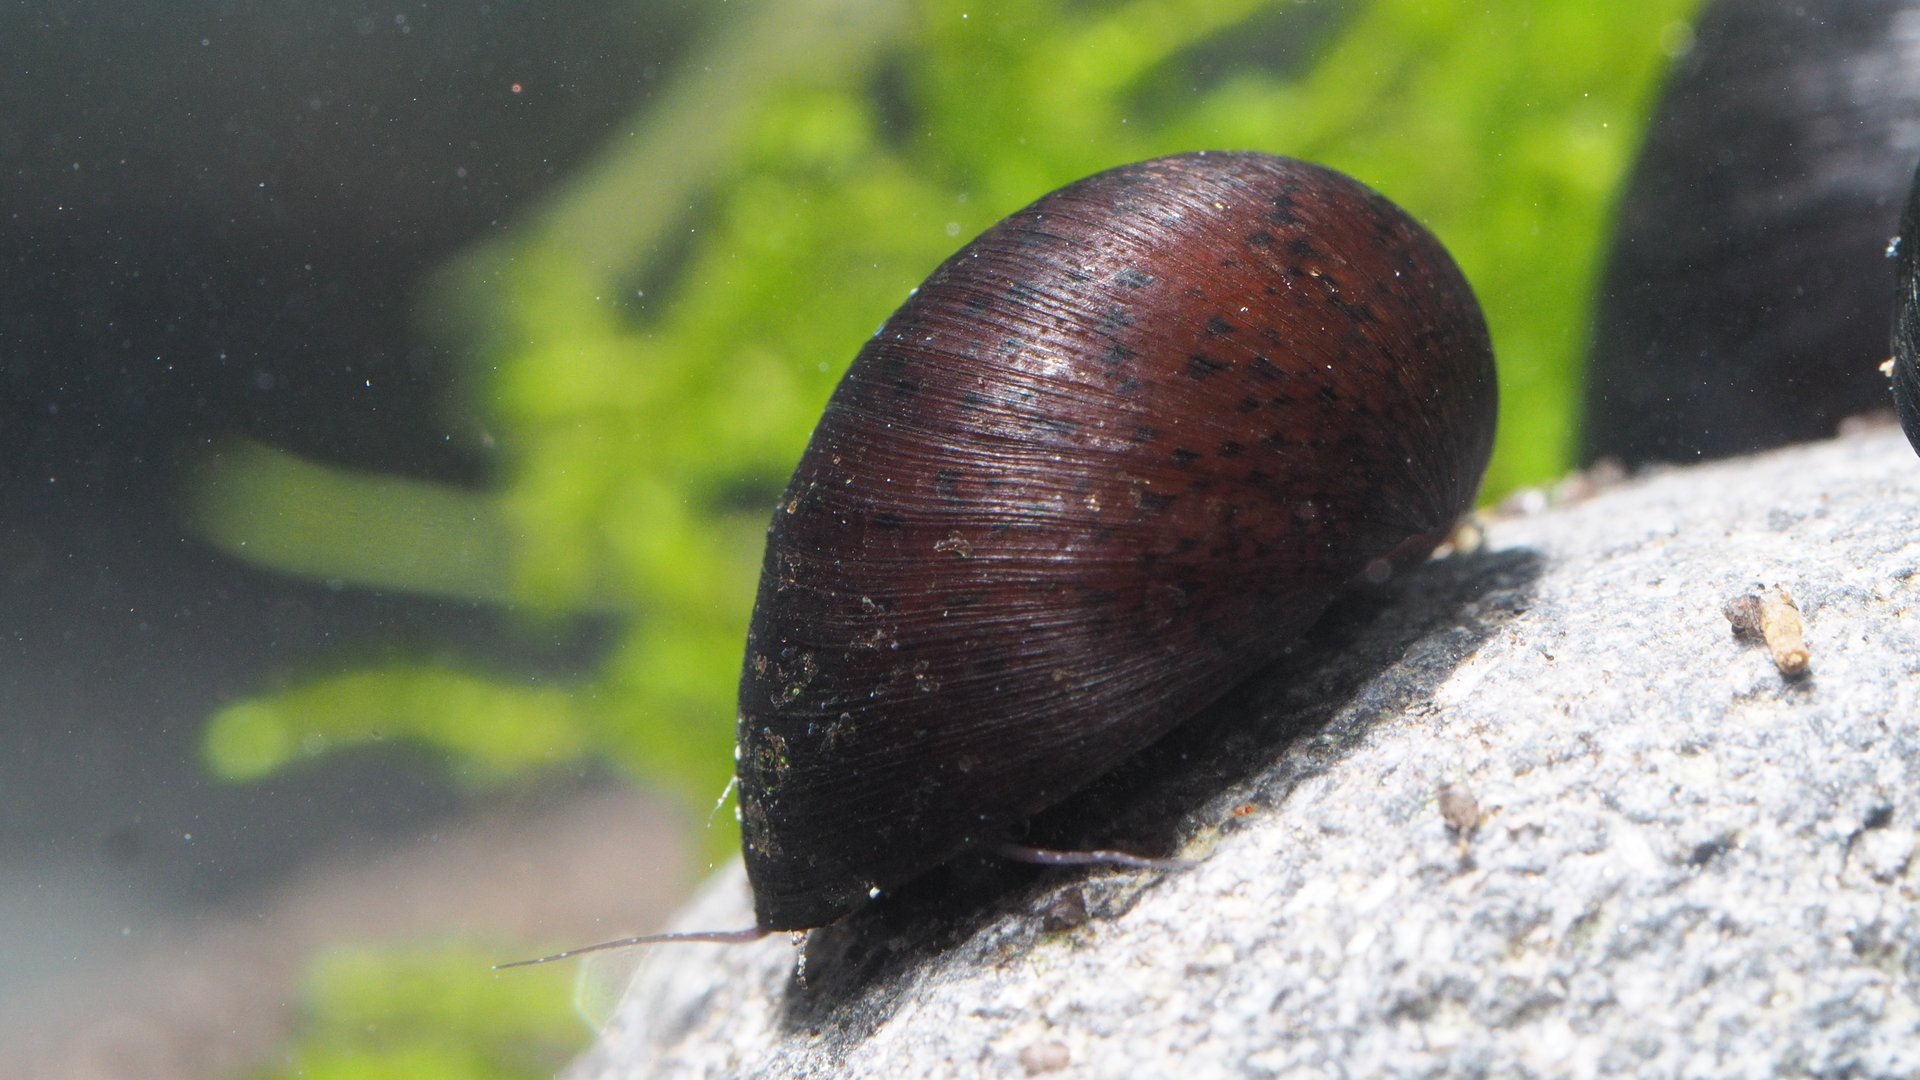
\includegraphics[width=0.7\linewidth]{abalone.jpg}
        \imageright{Garnelaxia}
    \end{figure}
\end{frame}

\end{document}
